\section{Hardware}
The following chapter deals with the hardware used for the cyberglove. It will explain how the new developed circuit board works and why certain decisions were made in this way. 

\subsection{Hardware selection and board design}
The old version of the cyberglove used an Arduino Uno board with a breakout chip for wireless data transmission. It also has an external battery in form of a typical smartphone power bank. Wiring is realized by a breadboard which is equipped with resistors and connects the glove with its components to the GPIO pins of the Arduino Uno. This setup needs a lot of space and is also heavy and unwieldy. In order to get a smaller and more light processing unit for the cyberglove, we need to develop a new hardware basis. The basic functions of the glove should be preserved, so we orient ourselves to the development of the original version. 

The Arduino Uno in the previous cyberglove uses a ATmega328 microprocessor which provides 16 MHz and a total amout of 20 GPIO pins, six of them are analog pins and the rest are for digital input and output. We decide to use the ATmega32U4 since it’s similar to the ATmega328 and can be programmed in the same way with the Arduino IDE. Just like the ATmega328, the ATmega32U4 has a clock frequency of 16 MHz and provides up to 32 I/O pins. 

We use an Li-Io battery cell with 1200 mAh to power the circuit board. The battery provides 3.7V, so we need a TPS63031 converter which converts the voltage to a constant 3.3V supply voltage for the ATmega32U4. Because we also want to charge the battery over our USB connector, we use the BQ24090 microchip to adjust the charging current. According to the following image, we set the maximum charging current to 500mA by installing a 1kOhm resistor.

\begin{figure}[!h]
	\centering
	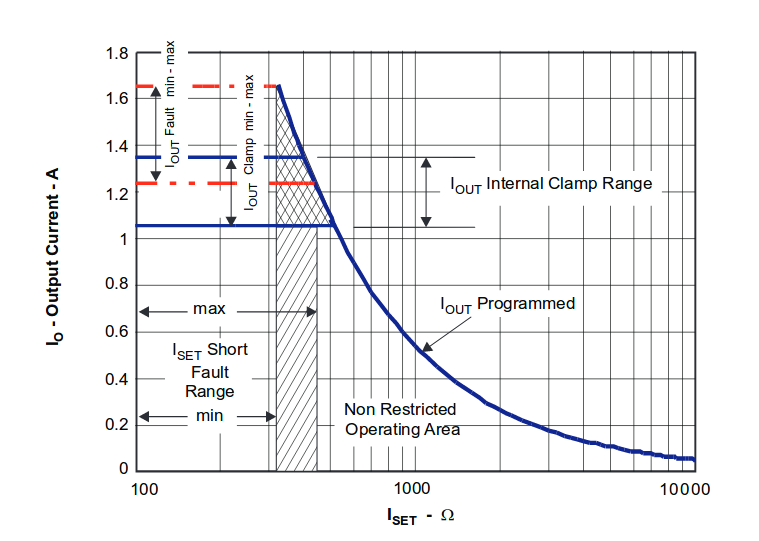
\includegraphics[width=\textwidth]{./images/image1.png}
	\caption{Programmed/Clamped Out Current}
	\label{img:grafik-dummy}
\end{figure}

After we soldered the board, we noticed that the battery was not charging. The measured charging curret is 150mA instead of our calculated 500mA. We were not able to track down the source of this error so this function will unfortunately be not available.

For the Wi-Fi connection we use the same ESP-12E module as the previous cyberglove used.
This way we could bui	lt up on the previous groups work and had the chance to improve it, instead of reinventing the data transfer, wasting resources.

The Wi-Fi module connects the hardware with the CAVE on startup and sends the evaluated output signal of the glove constantly to the CAVE server application.

After selecting the main hardware elements, we created a sketch in Eagle and wired the corresponding connections. Unfortunately, we made a spelling mistake with the USB connection of the microcontroller. That’s why there needs to be an additional connection between pin 7 “VBUS” and the USB connector “VUSB”. 

The final wiring can be seen in the images \ref{img:board1}, \ref{img:board2} and \ref{img:board3}.

\begin{figure}[!h]
	\centering
	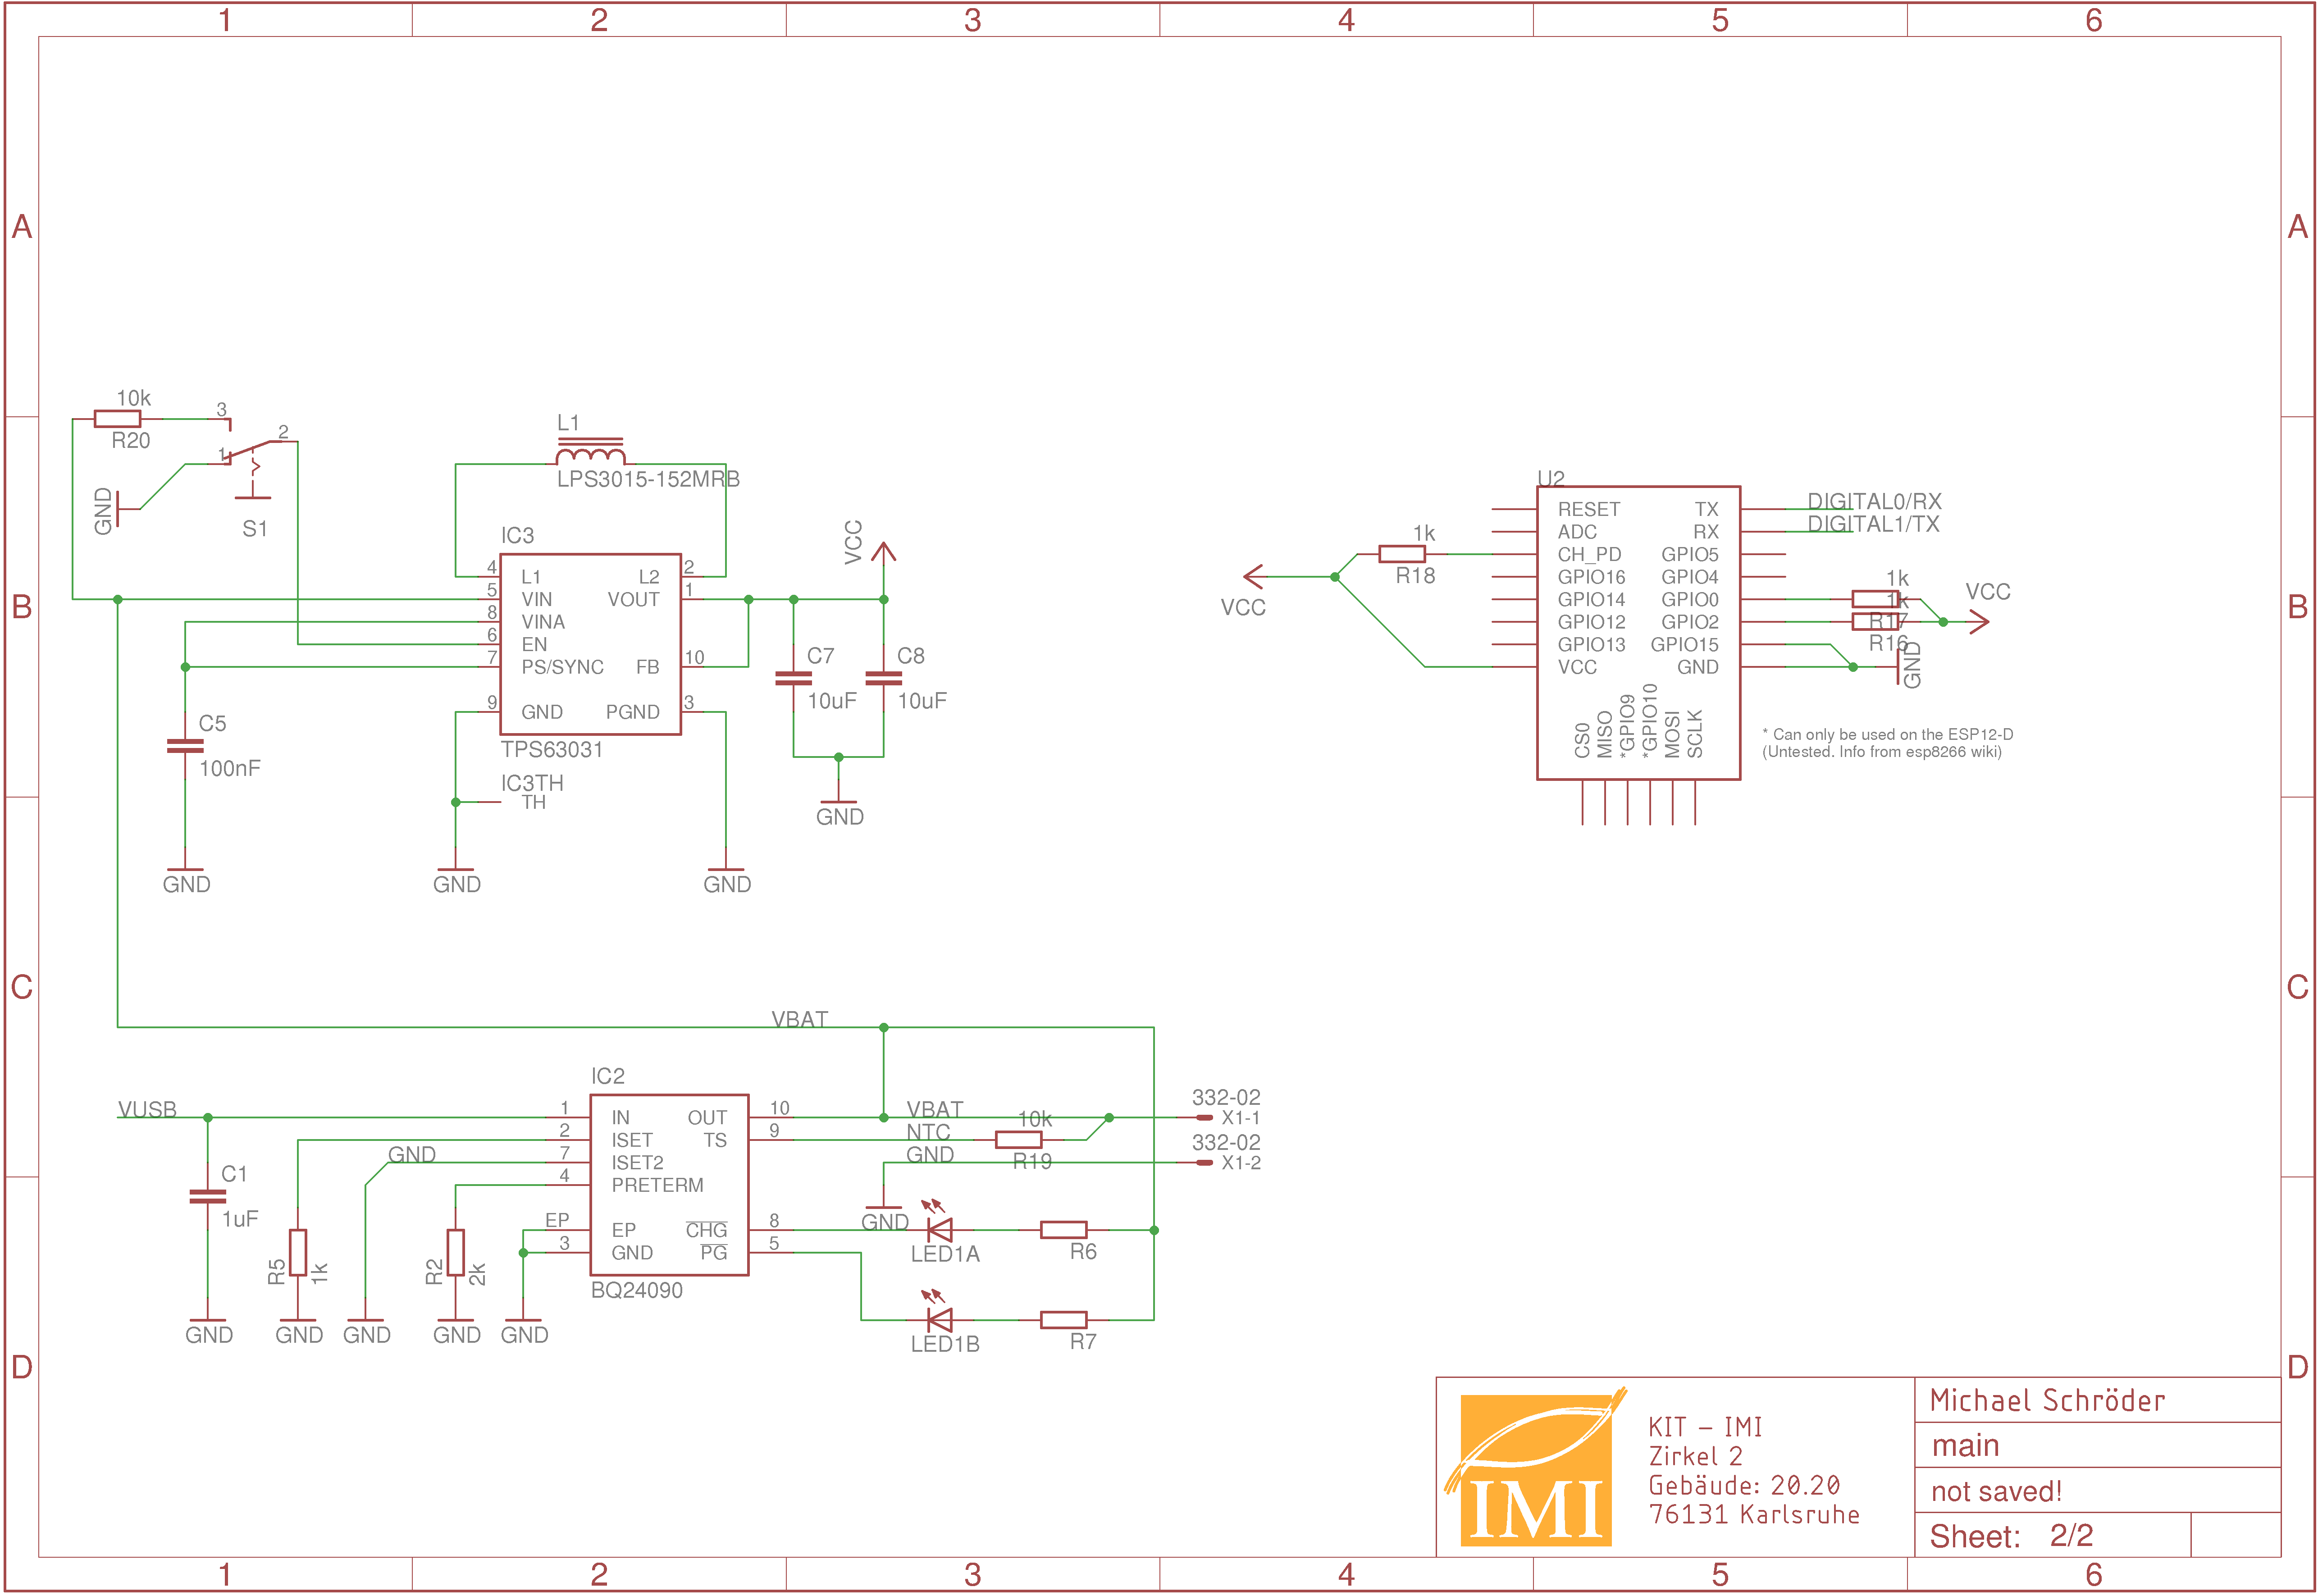
\includegraphics[width=.85\textwidth]{./images/image2.png}
	\caption{Final wiring of the board.}
	\label{img:board1}
\end{figure}
\begin{figure}[!h]
	\centering
	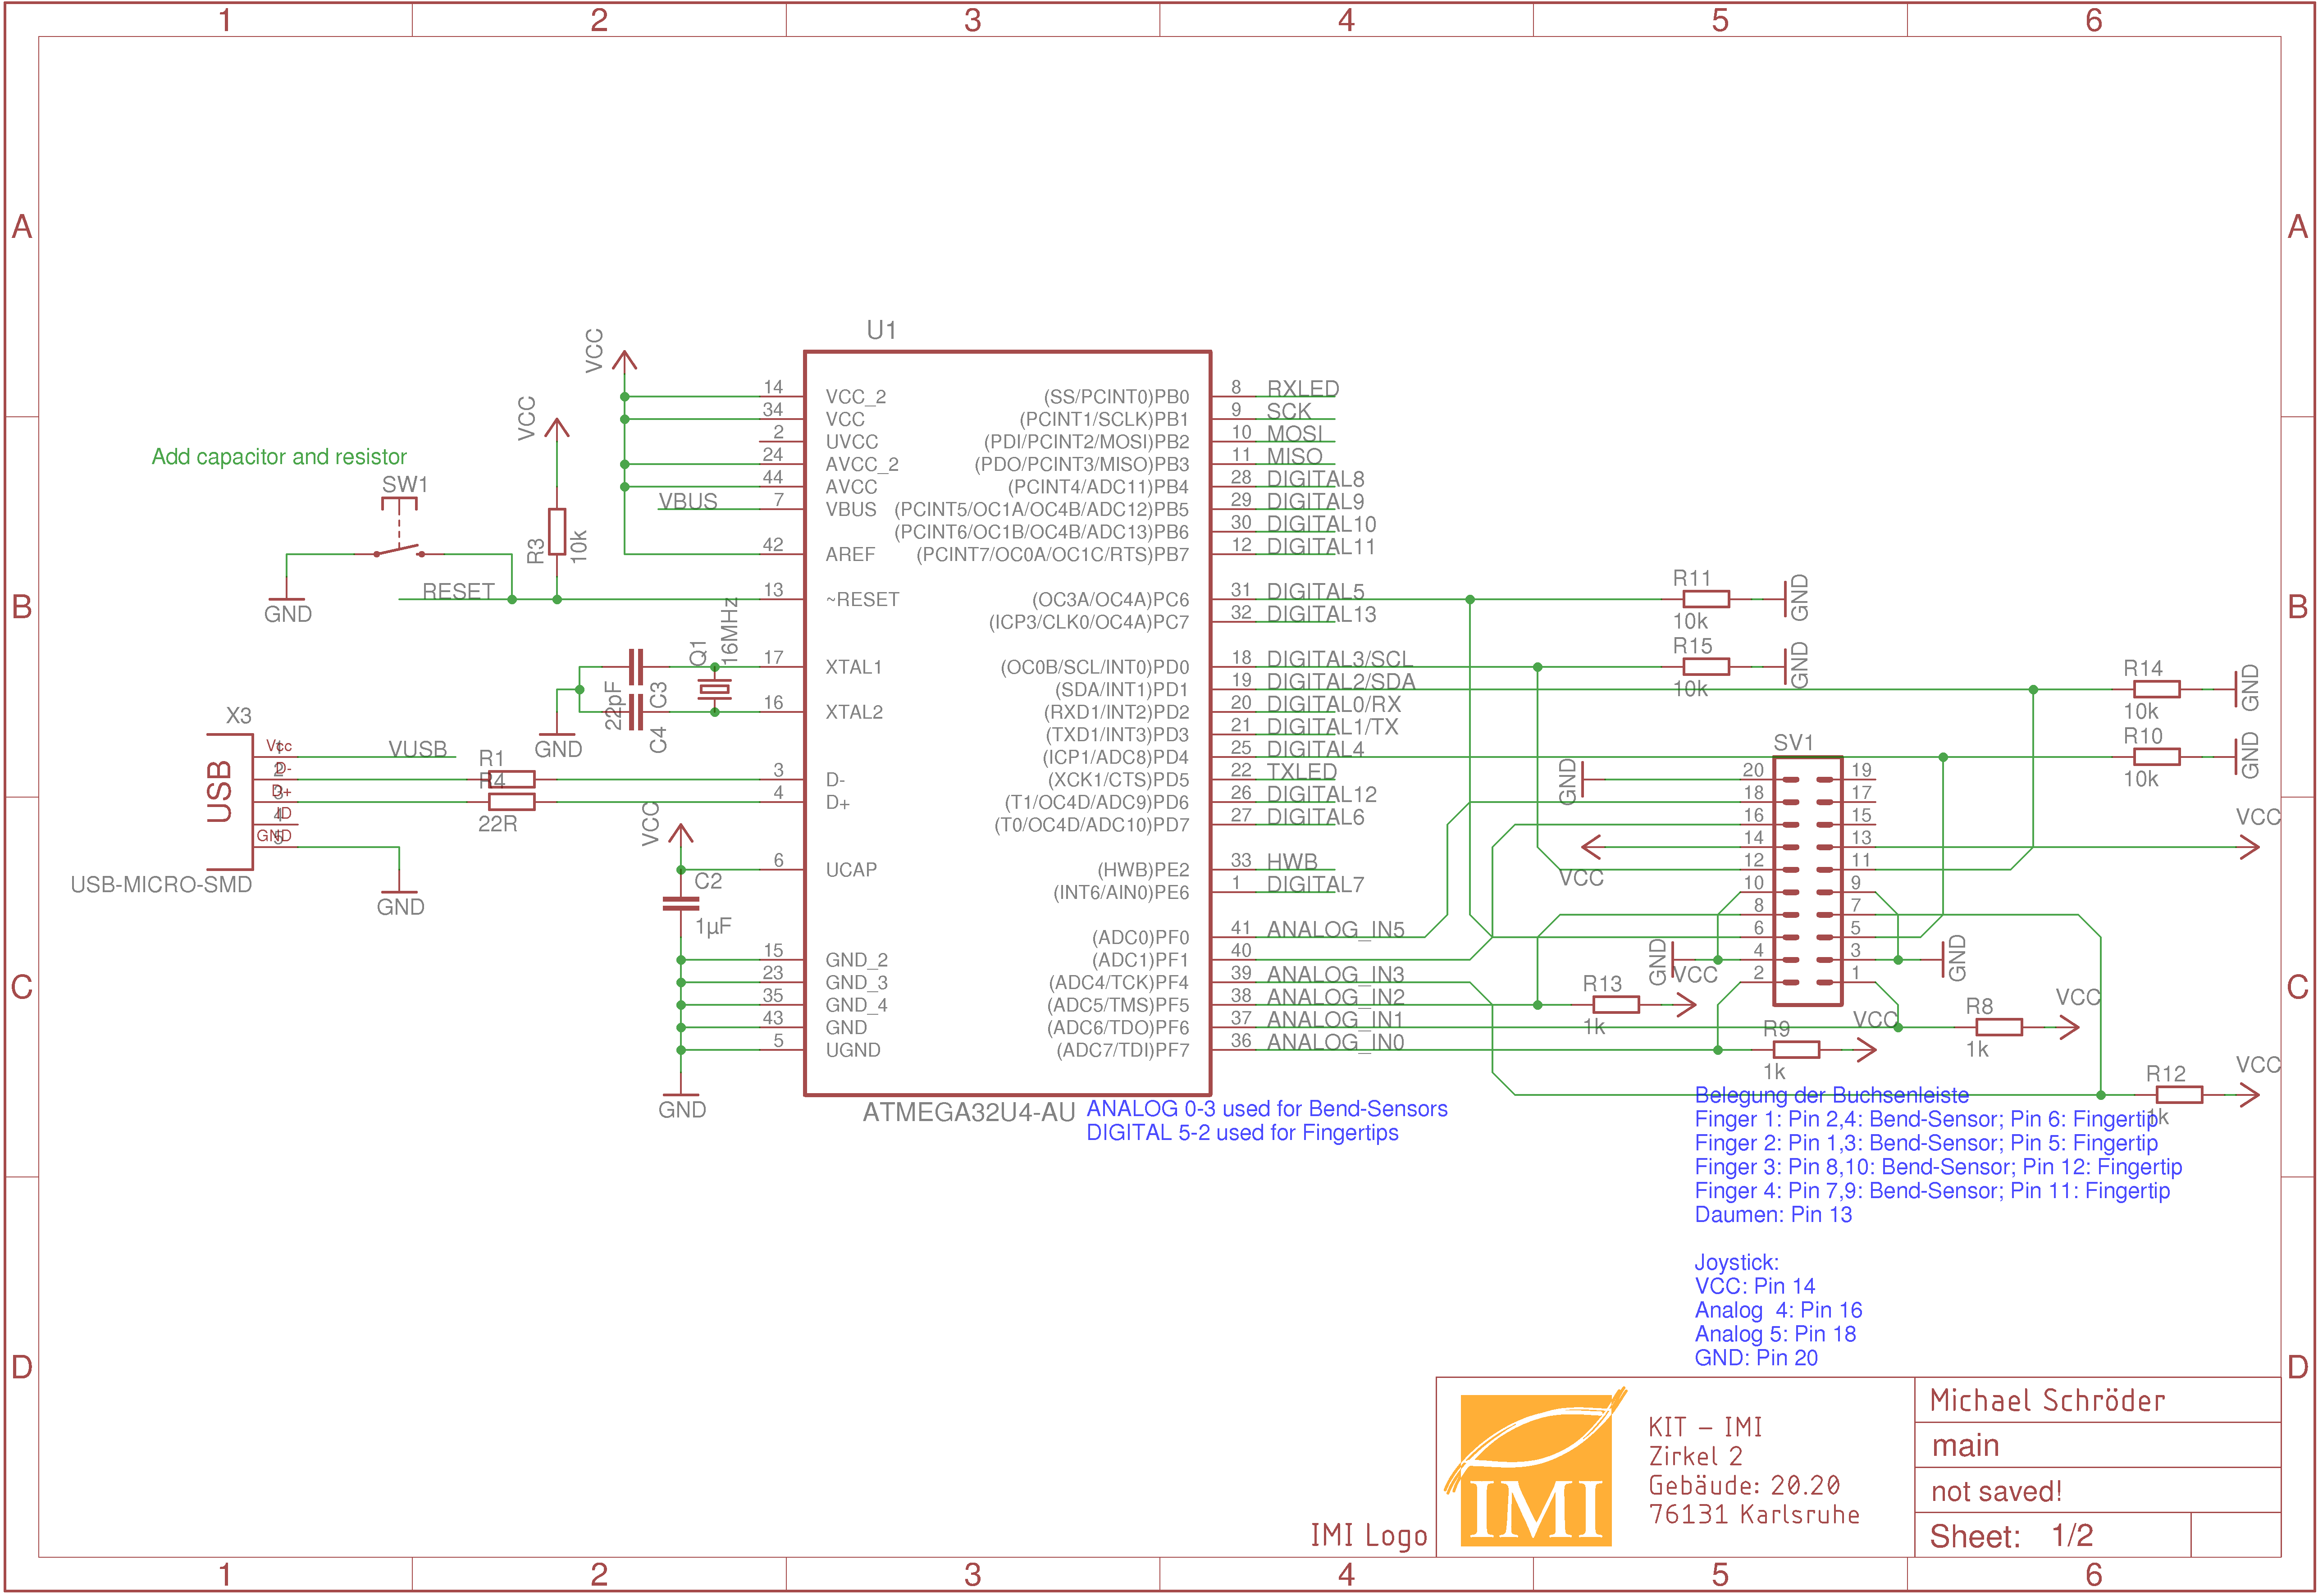
\includegraphics[width=.85\textwidth]{./images/image3.png}
	\caption{Final wiring of the board.}
	\label{img:board2}
\end{figure}
\begin{figure}[!h]
	\centering
	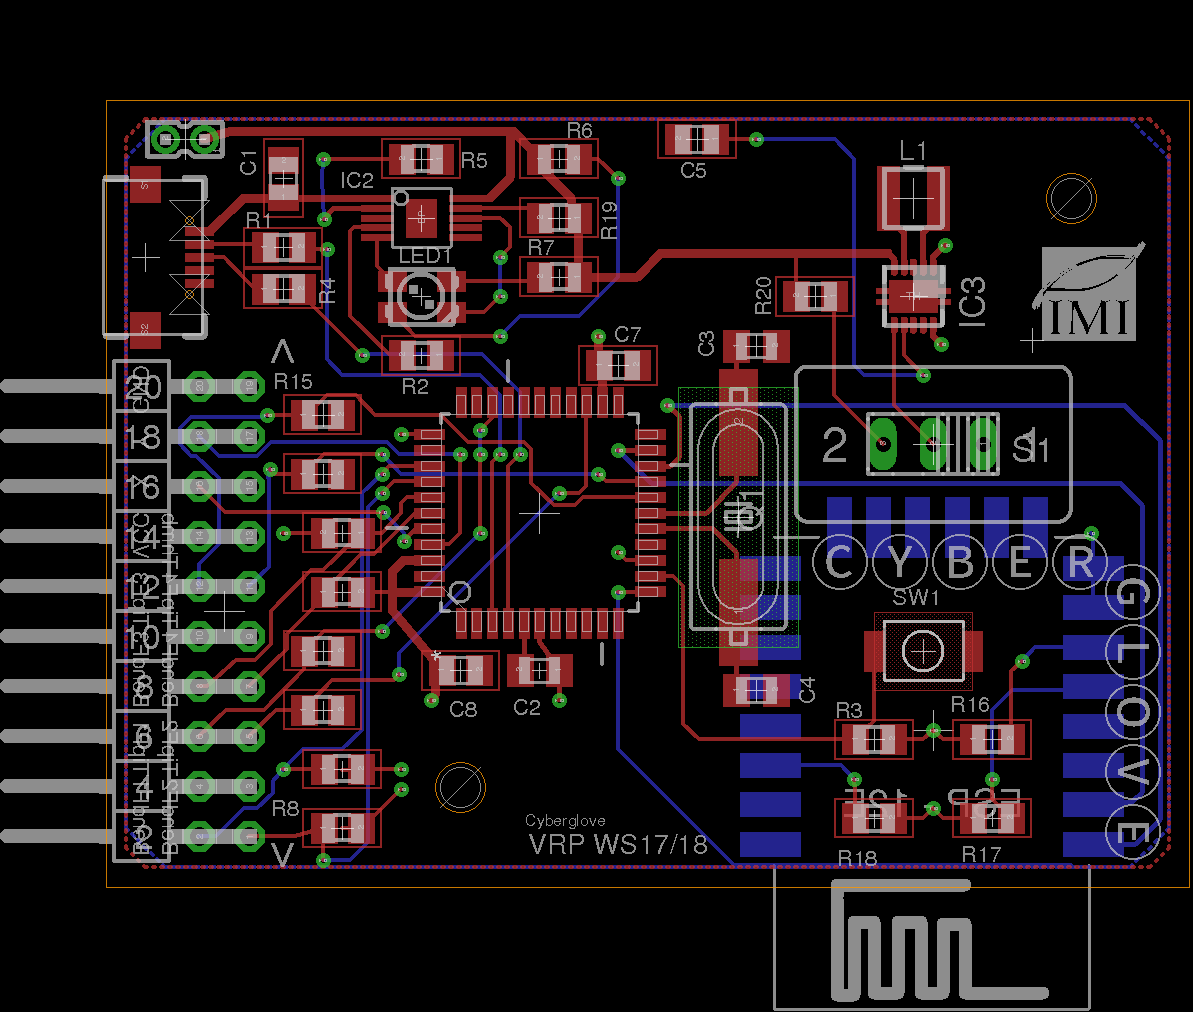
\includegraphics[width=.7\textwidth]{./images/image4.png}
	\caption{Final wiring of the board}
	\label{img:board3}
\end{figure}

We accidently destroyed the first board because the battery was turned upside down, which caused the TPS63031 to break. That’s why we had to solder another board. Using a diode would have avoided this problem because it only lets through the current in a predetermined direction and blocks the flow of current in case of accidental reverse polarity. 

We decided to use a bar of connector pins to connect the bendsensors and the fingercontacts with the circuit board. This allows the user to connect the glove with the board easily and disconnect both parts from each other for e.g. reprogramming the board without taking the glove itself with you. Image \ref{img:pins} shows the pin assignment of the pin bar.

\begin{figure}[!h]
	\centering
	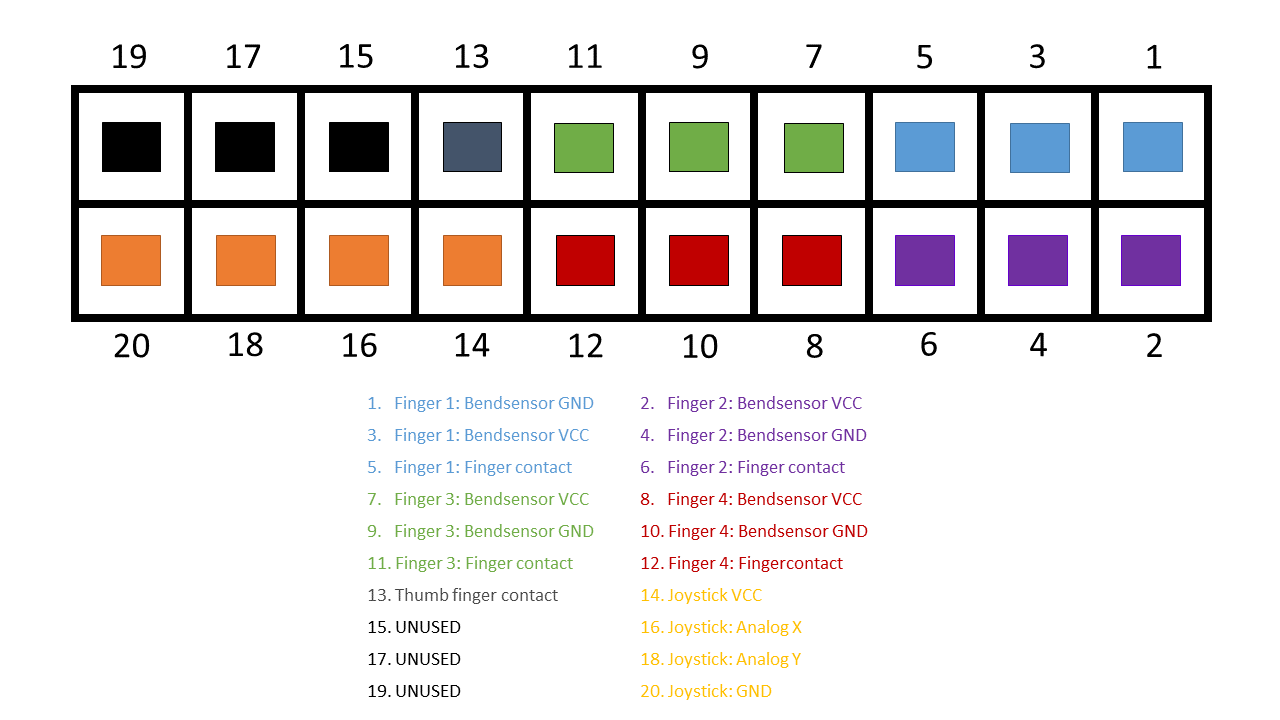
\includegraphics[width=\textwidth]{./images/image7.png}
	\caption{Assignment of the pin bar.}
	\label{img:pins}
\end{figure}


\subsection{The Cyberglove}

After soldering the hardware together, we could not communicate with the board yet, we first had to burn the bootloader in the Atmega chip. To do so we used a so-called programmer, soldered cables to the corresponding pins of the board, plugged these in the cables in the programmer and the programmer in the computer. With Amtel Studio we then could burn the bootloader and set the fuses, so that after that we could communicate with our board via USB as if it was an Arduino Leonardo.

\begin{figure}
	\begin{subfigure}{.5\textwidth}
		\centering
		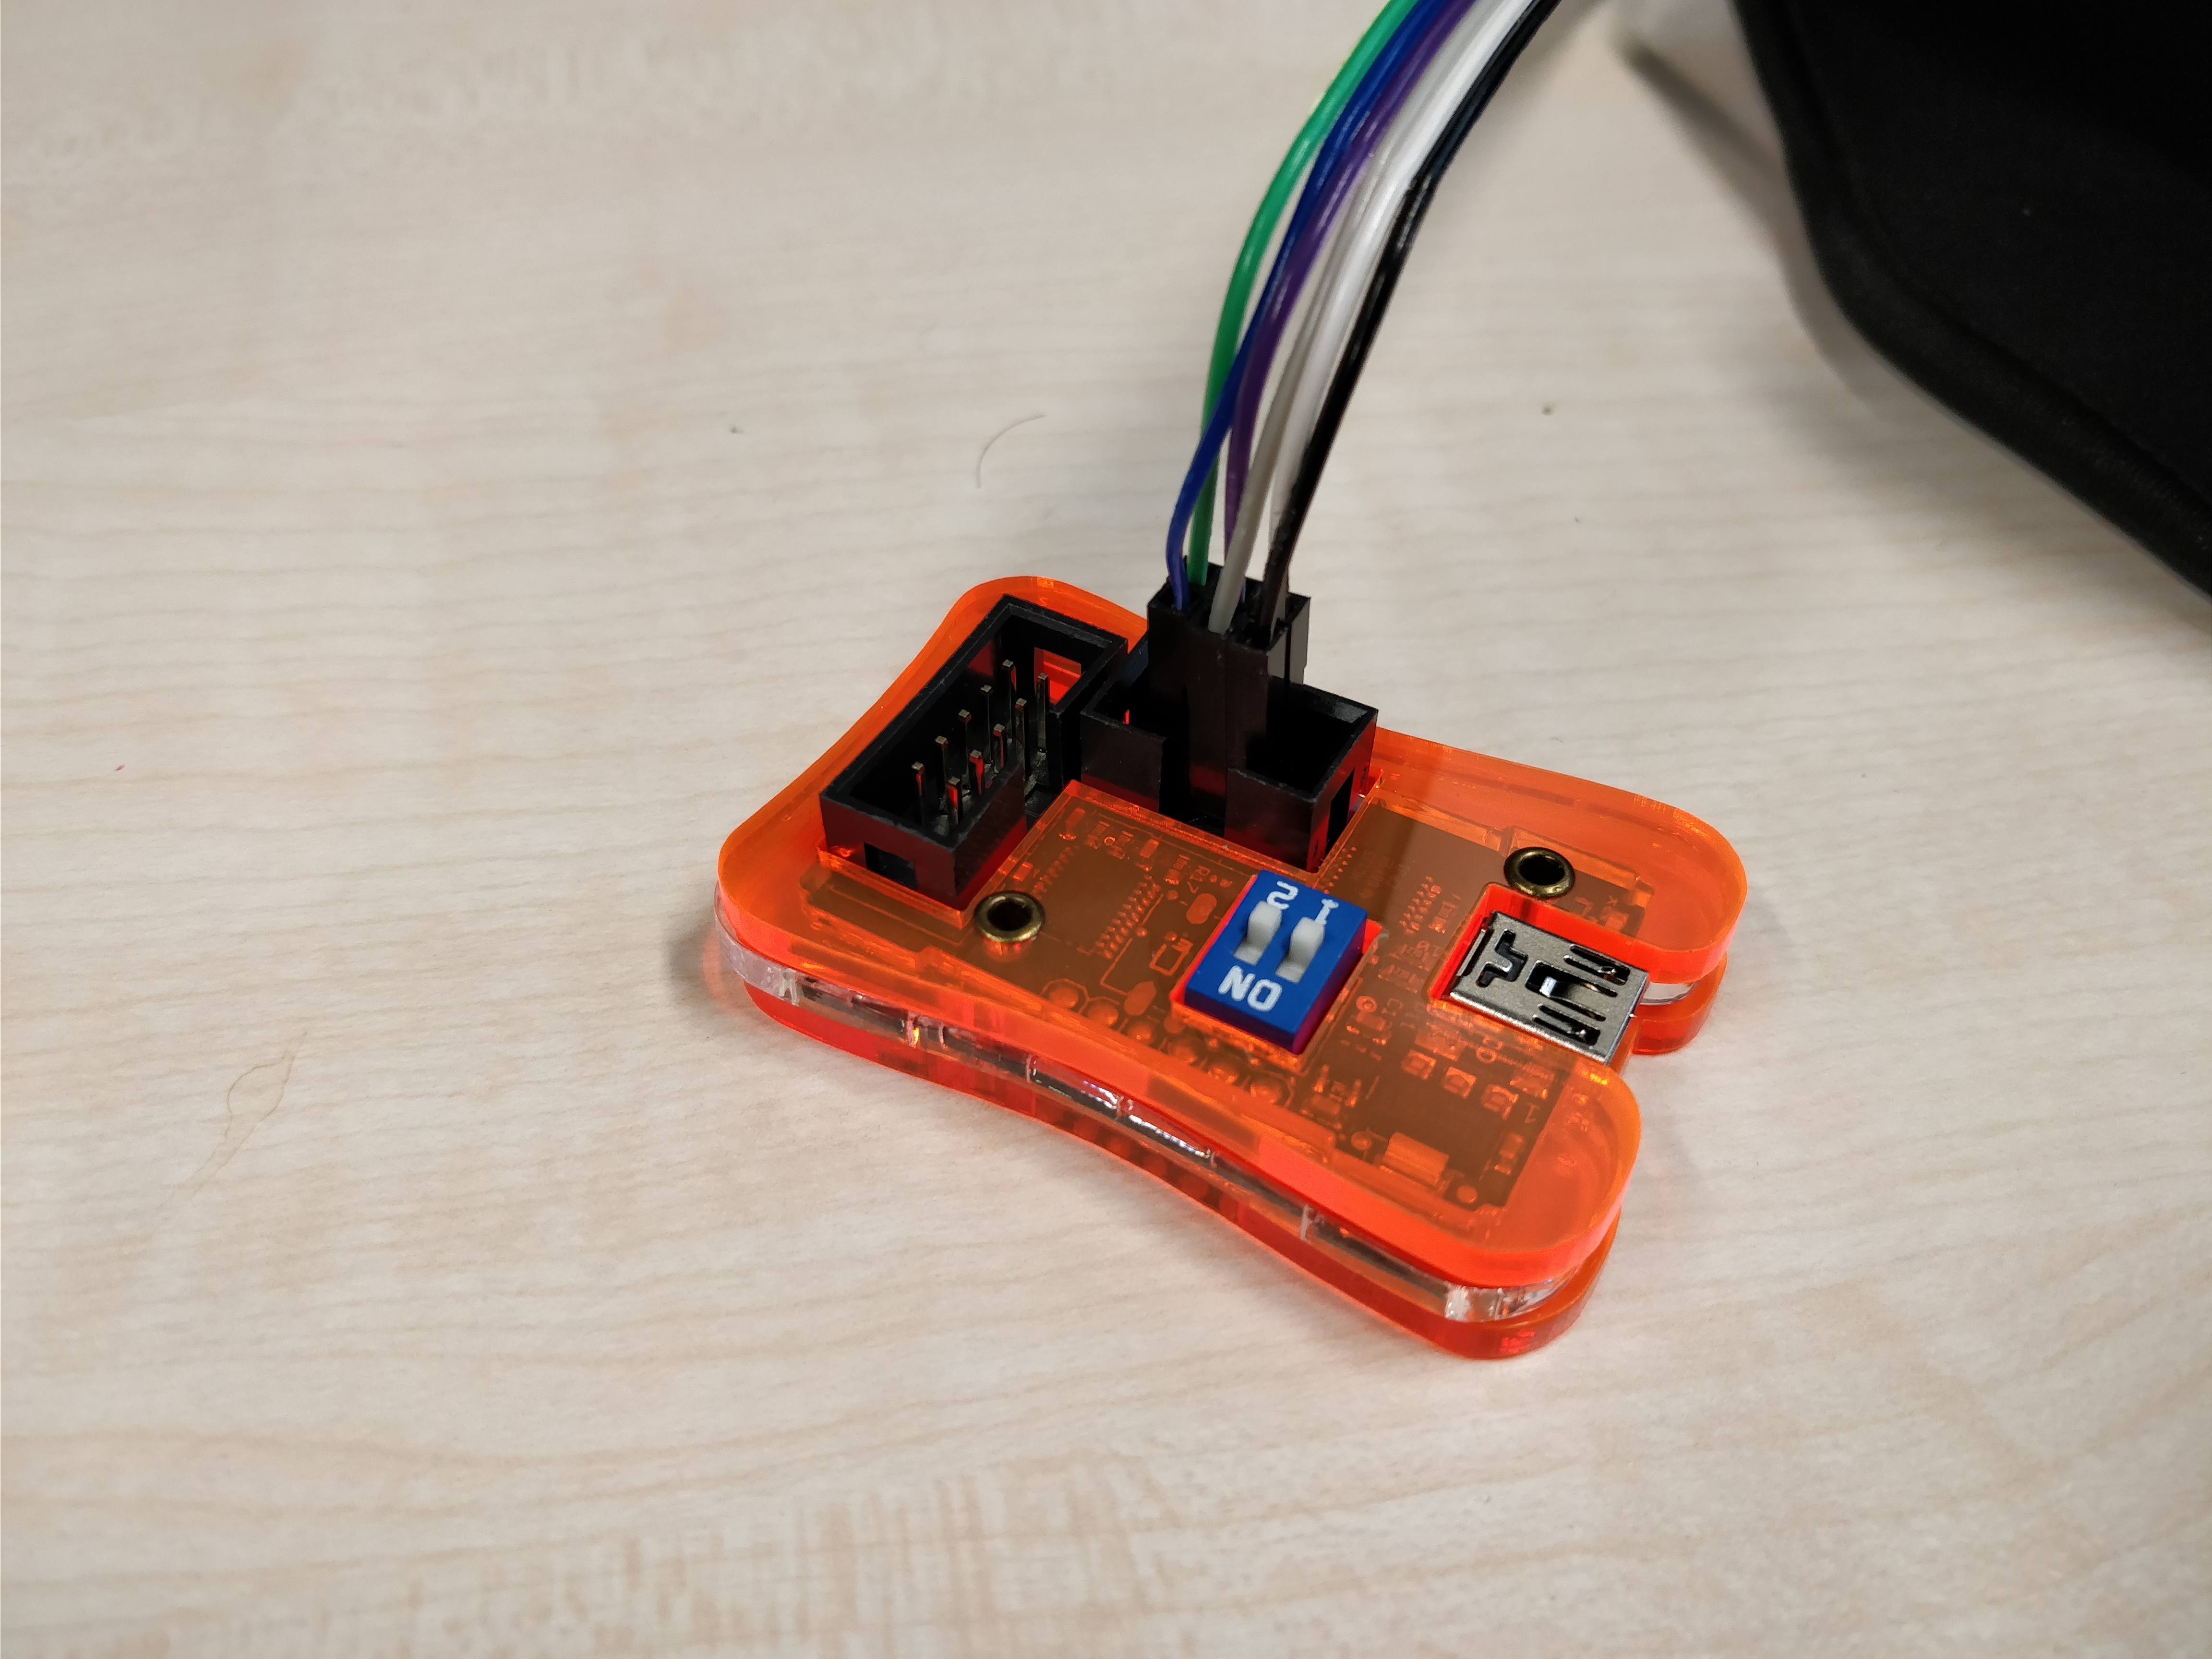
\includegraphics[width=.8\linewidth]{./images/image3.jpg}
	\end{subfigure}%
	\begin{subfigure}{.5\textwidth}
		\centering
		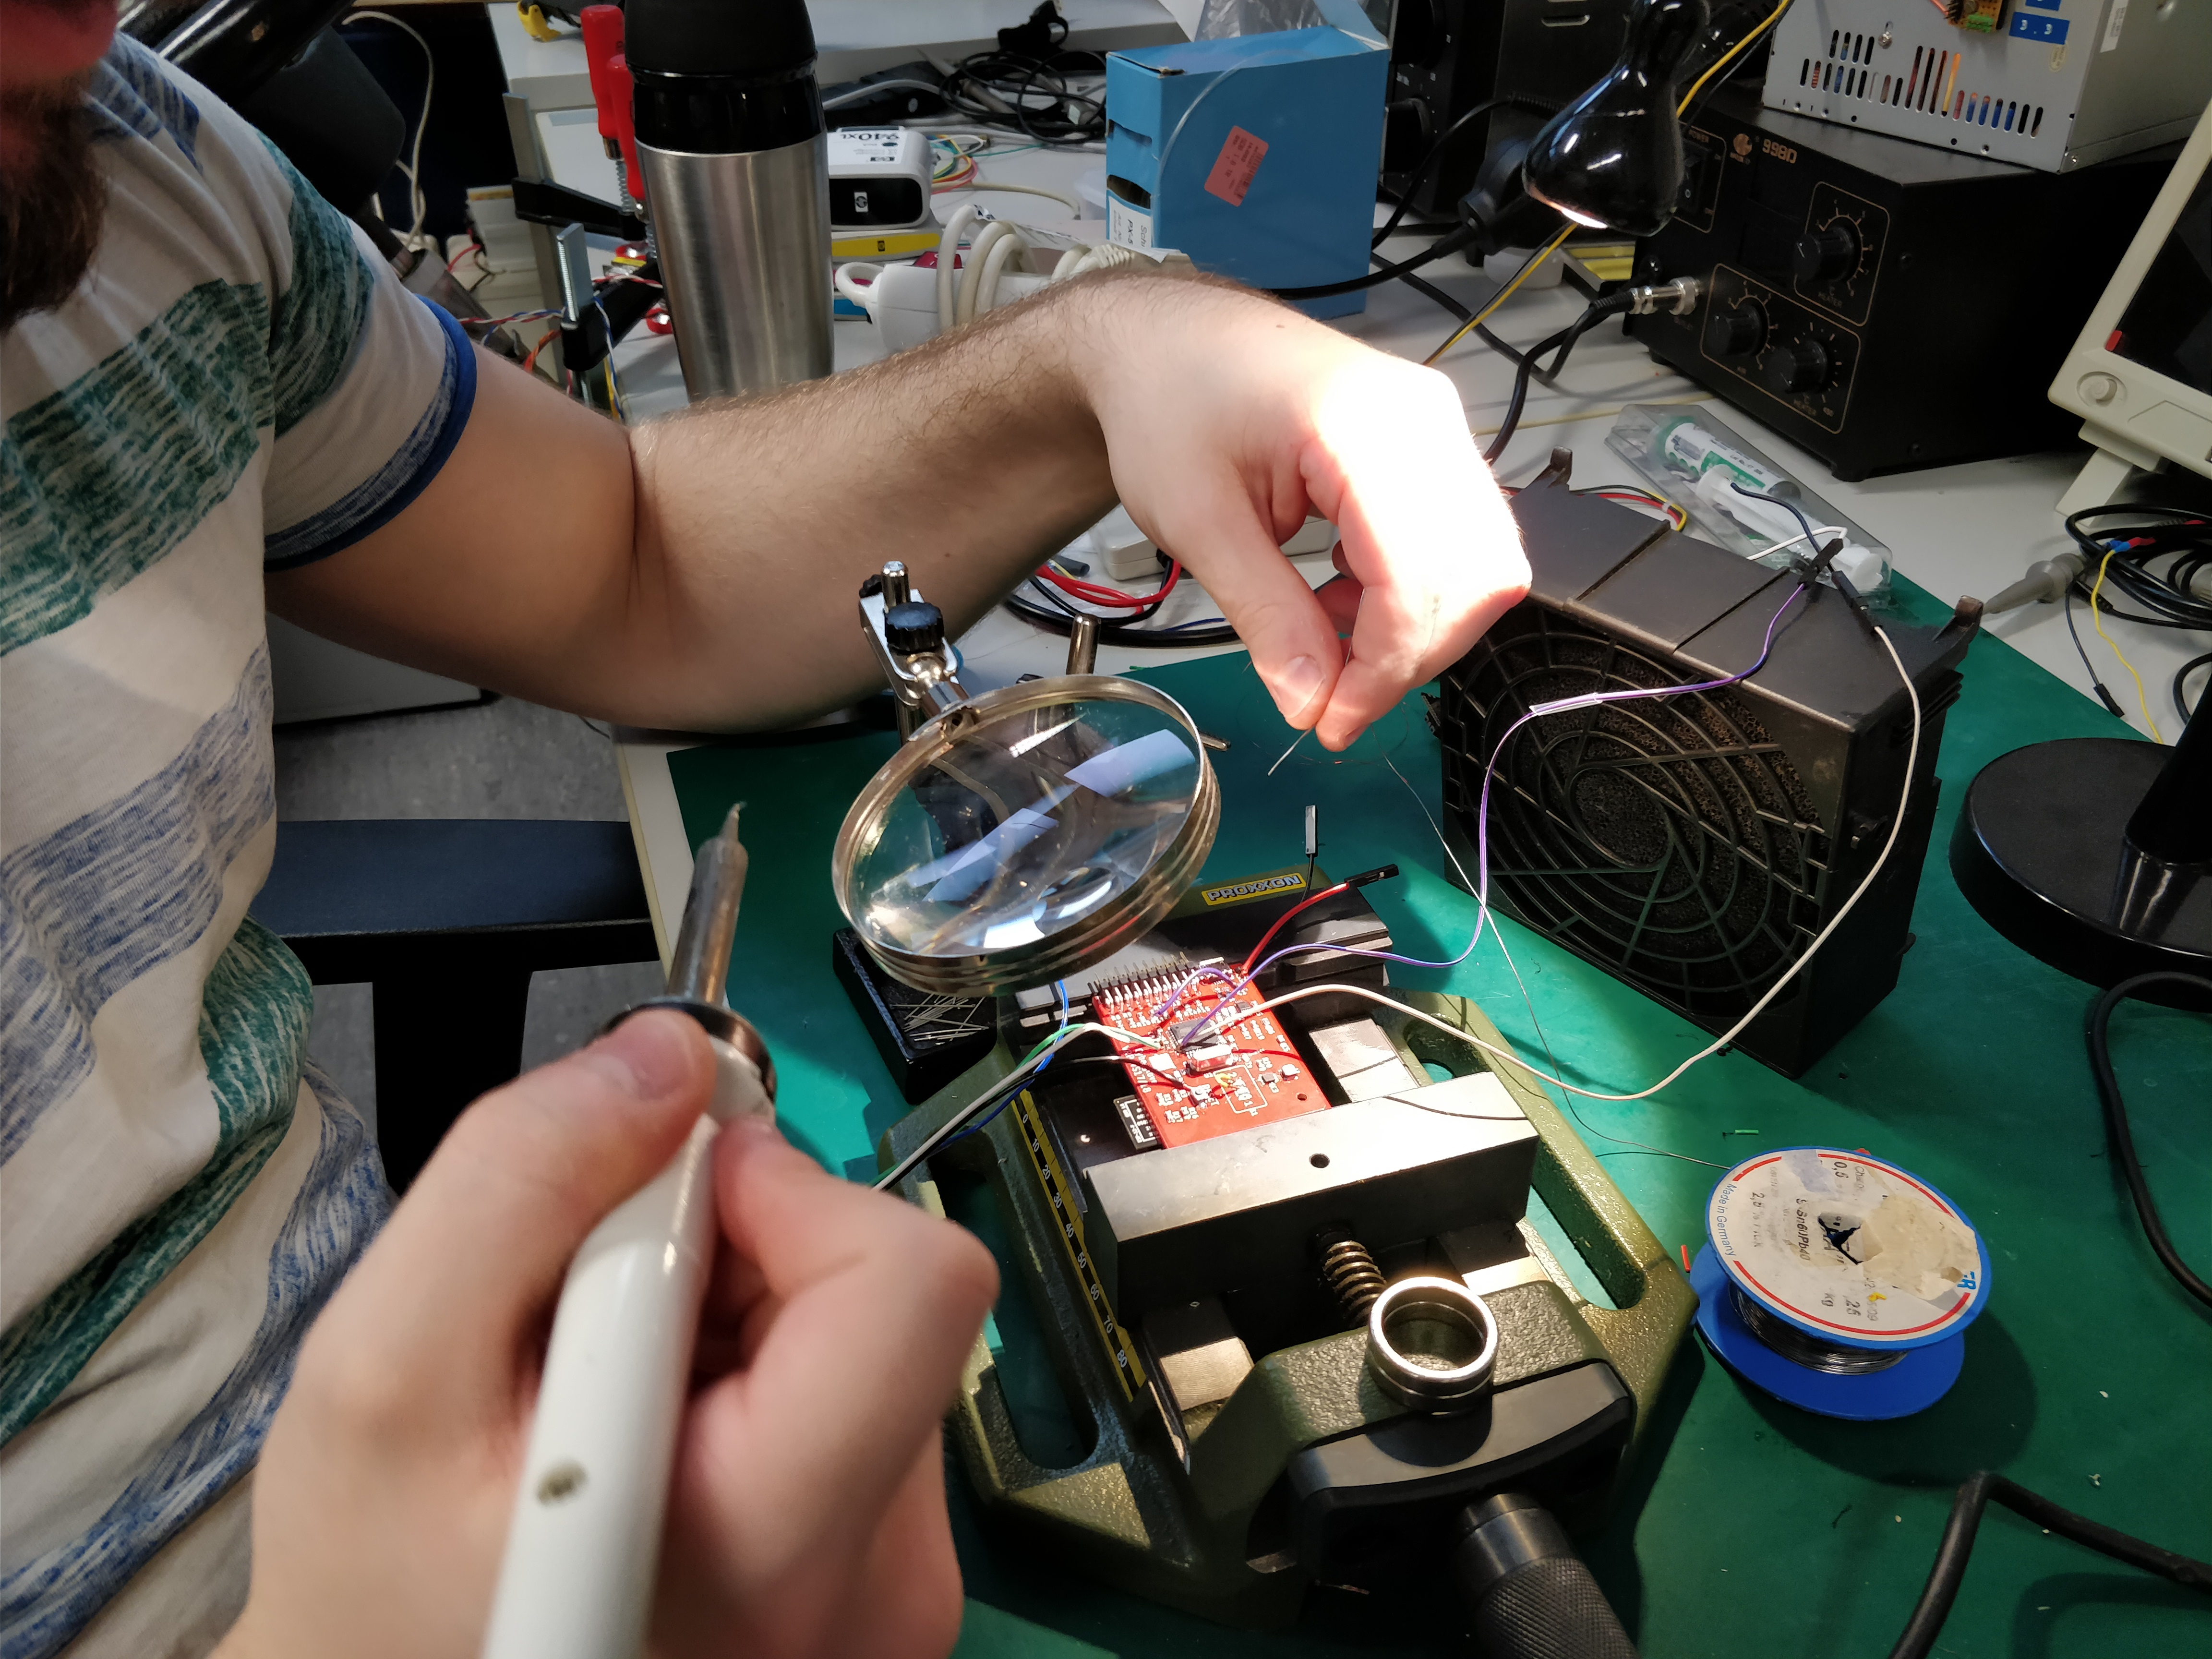
\includegraphics[width=.8\linewidth]{./images/image6.jpg}
	\end{subfigure}
	\begin{subfigure}{.5\textwidth}
		\centering
		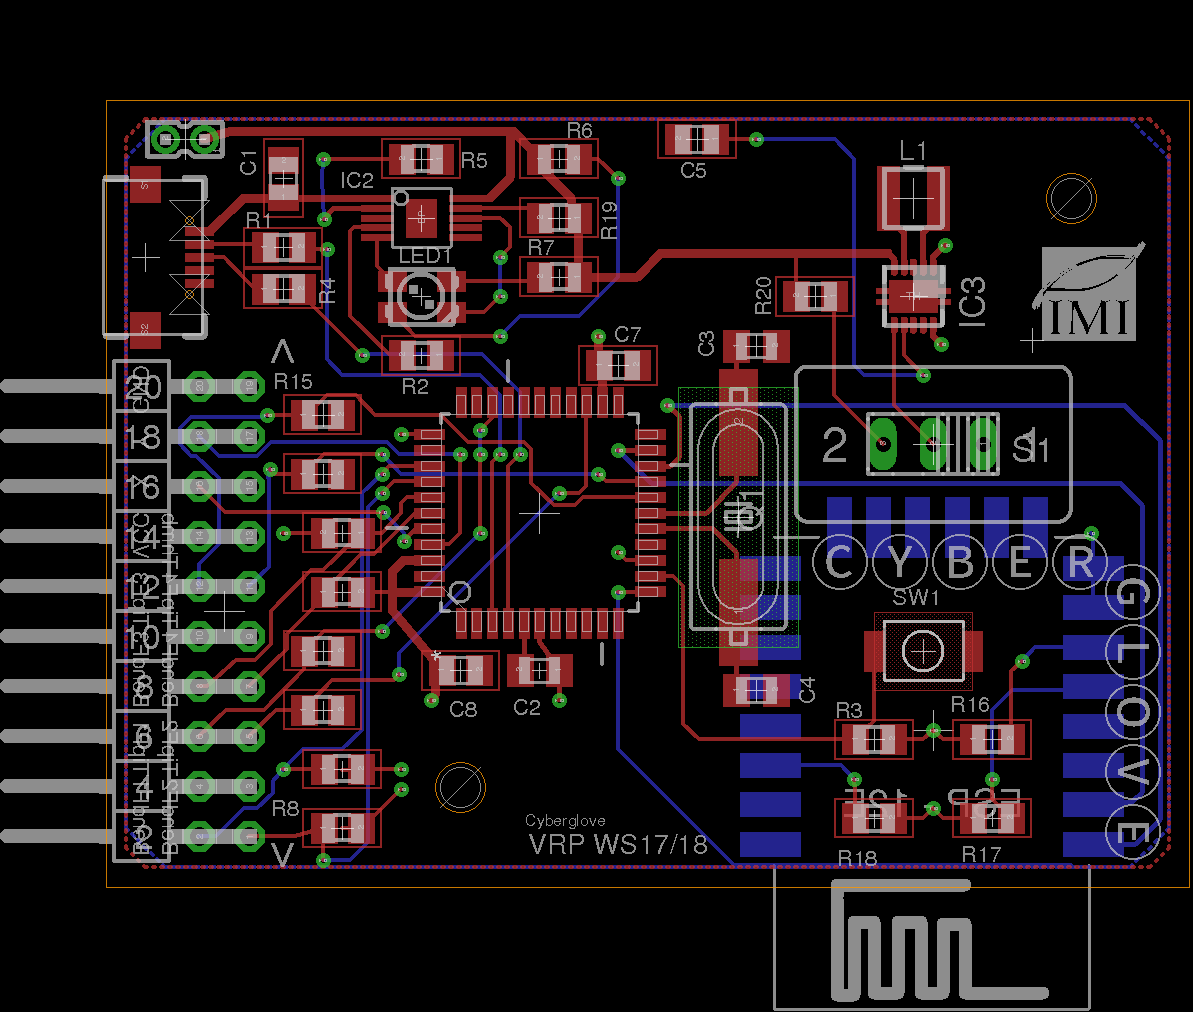
\includegraphics[width=.8\linewidth]{./images/image4.jpg}
	\end{subfigure}%
	\begin{subfigure}{.5\textwidth}
		\centering
		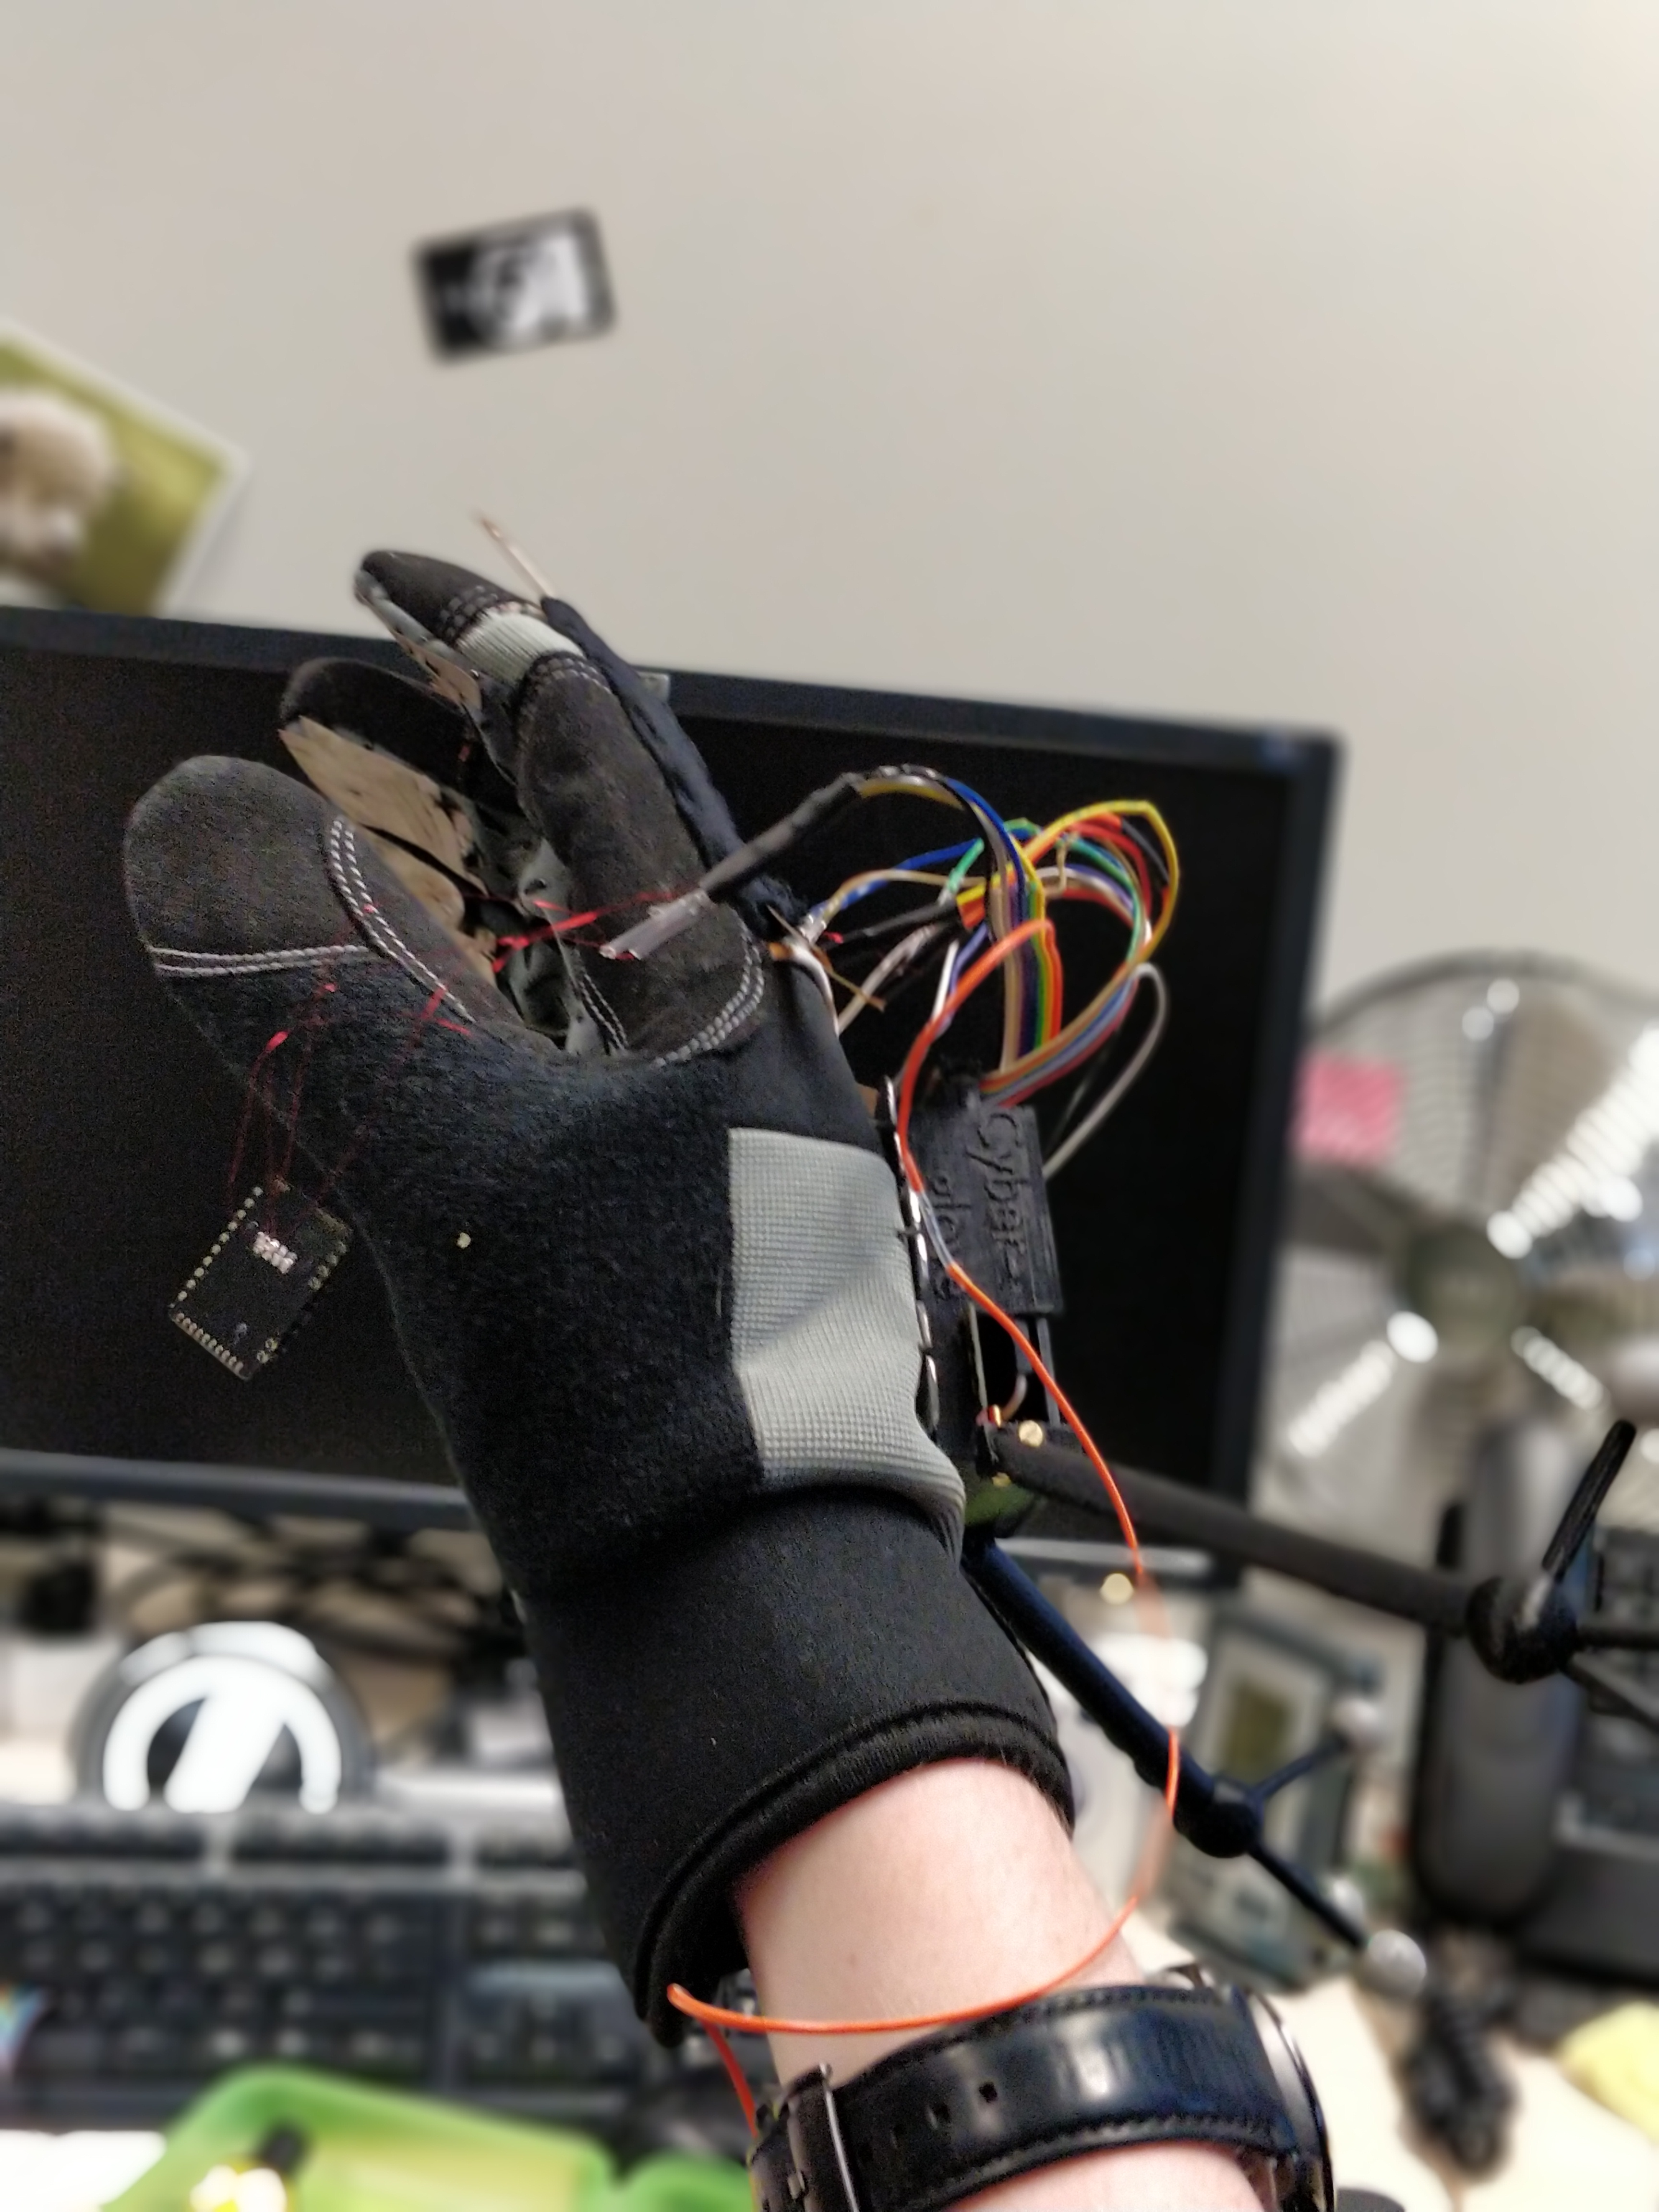
\includegraphics[width=.8\linewidth]{./images/image5.jpg}
	\end{subfigure}
	\caption{Work on the hardware.}
	\label{fig:photoshardware}
\end{figure}


\begin{figure}
	\begin{subfigure}{.5\textwidth}
		\centering
		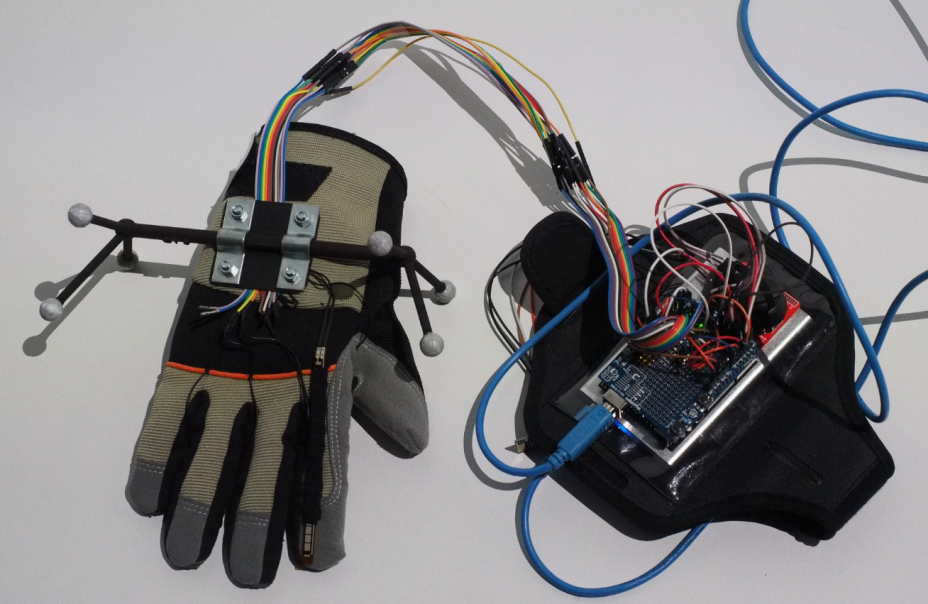
\includegraphics[width=.8\linewidth]{./images/image14.png}
	\end{subfigure}%
	\begin{subfigure}{.5\textwidth}
		\centering
		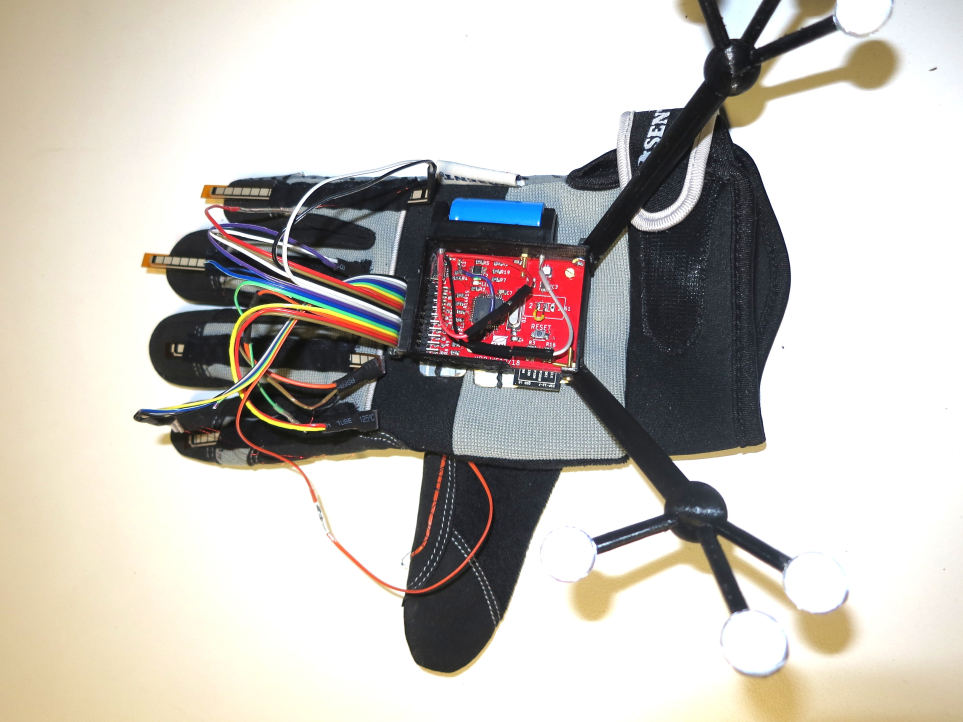
\includegraphics[width=.8\linewidth]{./images/image15.png}
	\end{subfigure}
	\caption{Comparison of the old and the new glove.}
	\label{fig:compare}
\end{figure}

The glove itself contains the following elements:
\begin{itemize}
	\item Fingercontacts on all fingers
	\item Four bendsensors
	\item A two-axis joystick
	\item Steel sheets for mounting the hardware case	
\end{itemize}

Putting the fingercontacts together with thumb closes the electric circuit and sends a “high” signal to the microcontroller. These signals can be used by the software to function as four buttons, one for each finger. If one of the bendsensors is bent this increases its resistance, which can be evaluated by the software. This makes it possible to recognize different gestures made by the glove. We decided to put steel sheets on the back of the glove, so the case of the board can be mounted with the help of magnets. 



\subsection{Case Design}
To design the case for the glove we used Blender, because it is easy to learn and to export. We started with a solid box of what size the final case should be, then made it hollow by subtracting a box the size of the board and and kept using the "boolean" operator to make holes for the pin header, wifi chip, etc. This way we also made a lid, which once fully inserted falls a millimetre to lock itself in place. After that we designed a housing for the flat battery which then could be inserted under the board. After discussing this design with the rest of the group we decided to discard this concept and instead attach a battery clip, which Michael provided, to the side of the case. For that we measured the exact position for the holes for screws and the pins on the clip and added appropriate holes to the model. We also found out we could not use the tracking of the old glove whith the new case because we could not mount it to the case. For this reason we designed two tracking arms which could be attached to the case and reused the tracking points of the old tracking mount. Other improvements to the case were pillars on which the board can rest and deepengings in which magnets can be placed to hold the case on the glove. 

Size adjustmends had to be made, which were rather difficult to achieve in Blender and we learned that while blender makes modeling of pleasing looking 3D objects easy, it is not designed to make precision models of parts and we should rather have used CAD. We did end up with a case which fits our needs but probably could have saved a lot of work in the process by using the right software.

\begin{figure}
	\centering
	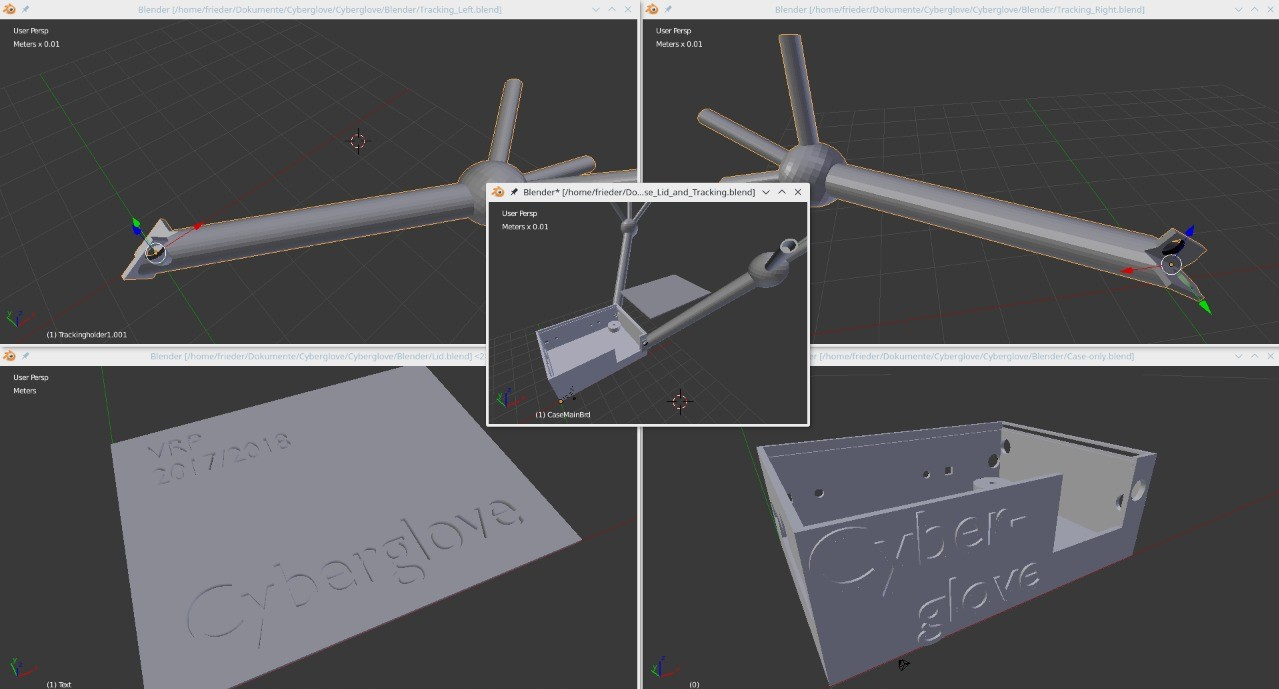
\includegraphics[width=\textwidth]{./Screenshots/Case-Screenshot.jpg}
	\caption{The case and its parts}
	\label{img:grafik-dummy}
\end{figure}